% figure1_matrix.tex — 2x3 time-x-tier matrix (revised).
%   Round 2 fixes per user feedback:
%   - Dashed tier bands removed (didn't make sense as borders).
%   - Vertical partitions added between Turn N | Idle | Turn N+1, with phase-flow
%     arrows above each partition.
%   - Promote arrow upgraded to a thick curved teal path from host2 -> gpu3,
%     clearly visible.
%   - Q_2 (next-turn signal) shown entering the middle column.
%   - Labels generalized: "Q_2" tagged with "next-turn signal".
% Shared preamble for standalone Figure 1 variants.
\documentclass[border=8pt,tikz]{standalone}
\usepackage{amsmath}
\usepackage{amssymb}
\usepackage{tikz}
\usetikzlibrary{arrows.meta,positioning,calc,fit,shapes.geometric,backgrounds}
\usepackage{xcolor}
\usepackage[T1]{fontenc}
\usepackage{mathptmx}
\newcommand{\repairkv}{\textsc{RepairKV}}
\newcommand{\bbase}{\ensuremath{B_{\mathrm{base}}}}
\newcommand{\bmatch}{\ensuremath{B_{\mathrm{match}}}}

\begin{document}
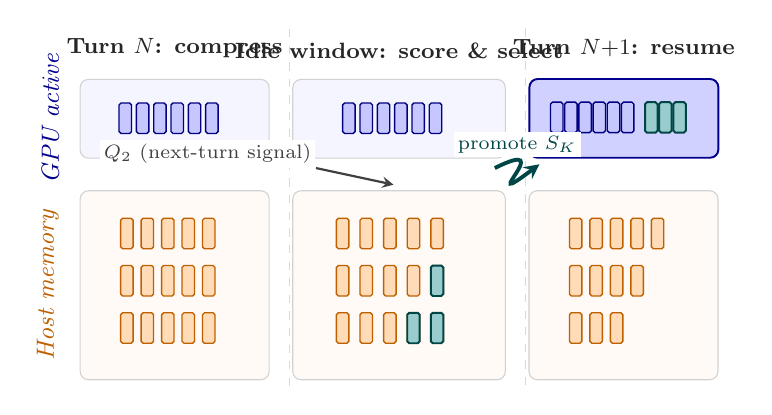
\begin{tikzpicture}[
  >=latex, line width=0.4pt,
  cell/.style={rounded corners=3pt, draw=gray!35, line width=0.4pt},
  gpucell/.style={cell, fill=blue!4},
  hostcell/.style={cell, fill=orange!4},
  activecell/.style={cell, fill=blue!18, draw=blue!55!black, line width=0.7pt},
  chip/.style={rounded corners=0.7pt, minimum width=4.5pt, minimum height=11pt,
               inner sep=0pt, line width=0.5pt},
  gpuchip/.style={chip, draw=blue!50!black, fill=blue!22},
  hostchip/.style={chip, draw=orange!75!black, fill=orange!28},
  promchip/.style={chip, draw=teal!55!black, fill=teal!40, line width=0.7pt},
  rowlabel/.style={font=\itshape\small, text=black!70},
  collabel/.style={font=\bfseries\footnotesize, align=center, text=black!85},
  anno/.style={font=\scriptsize, text=black!72, align=center},
  promarr/.style={->, line width=1.4pt, draw=teal!55!black, >=stealth},
  sigarr/.style={->, line width=0.8pt, draw=black!75, >=stealth},
  phasearr/.style={->, line width=0.7pt, draw=gray!55, >=stealth},
  arrlabel/.style={font=\scriptsize, fill=white, inner sep=1.5pt, text=black!75},
  partition/.style={draw=gray!30, line width=0.4pt, dashed}
]
  % --- Cells: 3 columns x 2 rows ---
  \node[gpucell, minimum width=2.4cm, minimum height=1.0cm,
        anchor=south west] (gpu1) at (0, 1.4) {};
  \node[gpucell, minimum width=2.7cm, minimum height=1.0cm,
        anchor=south west] (gpu2) at (2.7, 1.4) {};
  \node[activecell, minimum width=2.4cm, minimum height=1.0cm,
        anchor=south west] (gpu3) at (5.7, 1.4) {};
  \node[hostcell, minimum width=2.4cm, minimum height=2.4cm,
        anchor=north west] (host1) at (0, 1.0) {};
  \node[hostcell, minimum width=2.7cm, minimum height=2.4cm,
        anchor=north west] (host2) at (2.7, 1.0) {};
  \node[hostcell, minimum width=2.4cm, minimum height=2.4cm,
        anchor=north west] (host3) at (5.7, 1.0) {};

  % --- Tier labels (rotated, on left) ---
  \node[rowlabel, anchor=south, rotate=90, text=blue!55!black]
       at ([xshift=-4pt]gpu1.west) {GPU active};
  \node[rowlabel, anchor=south, rotate=90, text=orange!75!black]
       at ([xshift=-4pt]host1.west) {Host memory};

  % --- Column titles (single-line above their cells, well separated) ---
  \node[collabel, anchor=south] at ([yshift=4pt]gpu1.north)
       {Turn $N$: compress};
  \node[collabel, anchor=south] at ([yshift=4pt]gpu2.north)
       {Idle window: score \& select};
  \node[collabel, anchor=south] at ([yshift=4pt]gpu3.north)
       {Turn $N{+}1$: resume};

  % --- Vertical phase partitions (full height, solid thin) ---
  \draw[partition] ([xshift=-1pt, yshift=18pt]gpu2.north west) -- ([xshift=-1pt, yshift=-2pt]host2.south west);
  \draw[partition] ([xshift=-1pt, yshift=18pt]gpu3.north west) -- ([xshift=-1pt, yshift=-2pt]host3.south west);

  % --- GPU chips (B_base = 6 in cells 1,2; +3 promoted in cell 3) ---
  \foreach \i in {1,...,6}{
    \pgfmathsetmacro{\xa}{0.22*\i+0.36}
    \pgfmathsetmacro{\xb}{0.22*\i+0.50}
    \pgfmathsetmacro{\xc}{0.18*\i+0.18}
    \node[gpuchip] at ([xshift=\xa cm,yshift=-0.5cm]gpu1.north west) {};
    \node[gpuchip] at ([xshift=\xb cm,yshift=-0.5cm]gpu2.north west) {};
    \node[gpuchip] at ([xshift=\xc cm,yshift=-0.5cm]gpu3.north west) {};
  }
  \foreach \i in {1,2,3}{
    \pgfmathsetmacro{\xs}{0.18*6+0.18*\i+0.30}
    \node[promchip] at ([xshift=\xs cm,yshift=-0.5cm]gpu3.north west) {};
  }

  % --- Host chips (3 sub-rows of 5) ---
  \foreach \i in {1,...,5}{
    \foreach \r in {0,1,2}{
      \pgfmathsetmacro{\xh}{0.26*\i+0.34}
      \pgfmathsetmacro{\yh}{-0.55-0.6*\r}
      \node[hostchip] at ([xshift=\xh cm,yshift=\yh cm]host1.north west) {};
    }
  }
  \foreach \i in {1,...,5}{
    \foreach \r in {0,1,2}{
      \pgfmathsetmacro{\xh}{0.30*\i+0.34}
      \pgfmathsetmacro{\yh}{-0.55-0.6*\r}
      \node[hostchip] at ([xshift=\xh cm,yshift=\yh cm]host2.north west) {};
    }
  }
  \pgfmathsetmacro{\xPa}{0.30*4+0.34} \pgfmathsetmacro{\yPa}{-0.55-0.6*2}
  \pgfmathsetmacro{\xPb}{0.30*5+0.34} \pgfmathsetmacro{\yPb}{-0.55-0.6*1}
  \pgfmathsetmacro{\xPc}{0.30*5+0.34} \pgfmathsetmacro{\yPc}{-0.55-0.6*2}
  \node[promchip] at ([xshift=\xPa cm,yshift=\yPa cm]host2.north west) {};
  \node[promchip] at ([xshift=\xPb cm,yshift=\yPb cm]host2.north west) {};
  \node[promchip] at ([xshift=\xPc cm,yshift=\yPc cm]host2.north west) {};
  % cell 3 host: 12 chips (3 fewer)
  \foreach \i in {1,...,5}{
    \pgfmathsetmacro{\xh}{0.26*\i+0.34}
    \node[hostchip] at ([xshift=\xh cm,yshift=-0.55cm]host3.north west) {};
  }
  \foreach \i in {1,...,4}{
    \pgfmathsetmacro{\xh}{0.26*\i+0.34}
    \node[hostchip] at ([xshift=\xh cm,yshift=-1.15cm]host3.north west) {};
  }
  \foreach \i in {1,...,3}{
    \pgfmathsetmacro{\xh}{0.26*\i+0.34}
    \node[hostchip] at ([xshift=\xh cm,yshift=-1.75cm]host3.north west) {};
  }

  % --- Q_2 signal entering host2 from the row gap, label inline with arrow ---
  \draw[sigarr] ([xshift=-30pt, yshift=8pt]host2.north)
                -- ([xshift=-2pt, yshift=2pt]host2.north);
  \node[arrlabel, anchor=south east]
        at ([xshift=-30pt, yshift=8pt]host2.north) {$Q_2$ (next-turn signal)};

  % --- Promote arrow: thick teal curve from host2 right edge -> gpu3 left edge ---
  \draw[promarr] ([xshift=-4pt, yshift=8pt]host2.north east)
       .. controls ([xshift=20pt, yshift=20pt]host2.north east)
                  and ([xshift=-20pt, yshift=-20pt]gpu3.south west) ..
       ([xshift=4pt, yshift=-2pt]gpu3.south west);
  \node[arrlabel, text=teal!55!black, anchor=south]
        at ($(host2.north east)!0.5!(gpu3.south west) + (0, 6pt)$)
        {promote $S_K$};
\end{tikzpicture}
\end{document}
